\section{Tutoring e gestione studenti internazionali}
Un aspetto fondamentale e particolarmente arricchente del mio tirocinio è stato il ruolo educativo e di tutoring. Ricoprire la posizione di formatore all'interno del Fablab ha rappresentato un'occasione unica per affinare le mie soft skills, mettendomi alla prova nella gestione di studenti, nel trasferimento tecnologico e nella comunicazione interculturale, dovendomi interfacciare con diversi gruppi di studenti internazionali provenienti da Bulgaria, Cipro e Ungheria parlando in inglese.

Il mio obiettivo principale non è stato solo quello di insegnare l'utilizzo passivo dei software o dei macchinari, ma di trasmettere una vera e propria metodologia progettuale (dal concetto al prodotto finito), modulando il livello tecnico delle lezioni in base al background dei ragazzi.

Questa esperienza di tutoring mi ha insegnato a tradurre concetti ingegneristici complessi in lezioni accessibili e stimolanti. Gestire le tempistiche, preparare il materiale di supporto (come presentazioni e file pre-impostati), preparare gli spazi di lavoro e risolvere gli imprevisti tecnici in tempo reale durante i workshop ha migliorato esponenzialmente le mie capacità organizzative e di project management.

%
\subsection{Comunicazione e barriere linguistiche}
L'interazione costante con i gruppi internazionali ha rappresentato, inoltre, uno straordinario banco di prova per le mie capacità comunicative e linguistiche. Dovendomi interfacciare quotidianamente in lingua inglese, ho migliorato notevolmente la mia fluidità espressiva, arricchendo in particolar modo il mio vocabolario legato all'inglese tecnico, riguardante termini rilevanti all'ingegneria, al software e alla meccanica. Ho imparato ad adattare rapidamente il mio registro linguistico, utilizzando esempi pratici e supporti visivi per superare le barriere linguistiche e mantenere alta l'attenzione e il coinvolgimento degli studenti.

\progetto{Ingegneria civile e topografica}{Gruppo Bulgari, Apr 2026}
Con i gruppi bulgari ho affrontato percorsi formativi su più livelli. Inizialmente, ho tenuto workshop focalizzati sul disegno tecnico e sul reverse engineering, spiegando loro come si concepiscono componenti in ottica industriale e professionale.
In una fase successiva, ho seguito un gruppo specifico orientato all'architettura e all'ingegneria civile. Con loro ho utilizzato AutoCAD, Solidworks e Sketchup: partendo dallo studio del terreno e dall'analisi delle curve di livello di una collina, abbiamo modellato in 3D l'intera pianta architettonica e la vista topografica. Il progetto è culminato con la stampa di complessi plastici architettonici in PLA bianco, pensati per essere successivamente dipinti e rifiniti a mano dagli studenti.
\\ Vedi figure \ref{fig:arch1}, \ref{fig:arch2} e \ref{fig:arch3}.
\begin{figure}
    \centering
    \begin{subfigure}{0.6\linewidth}
        \centering
        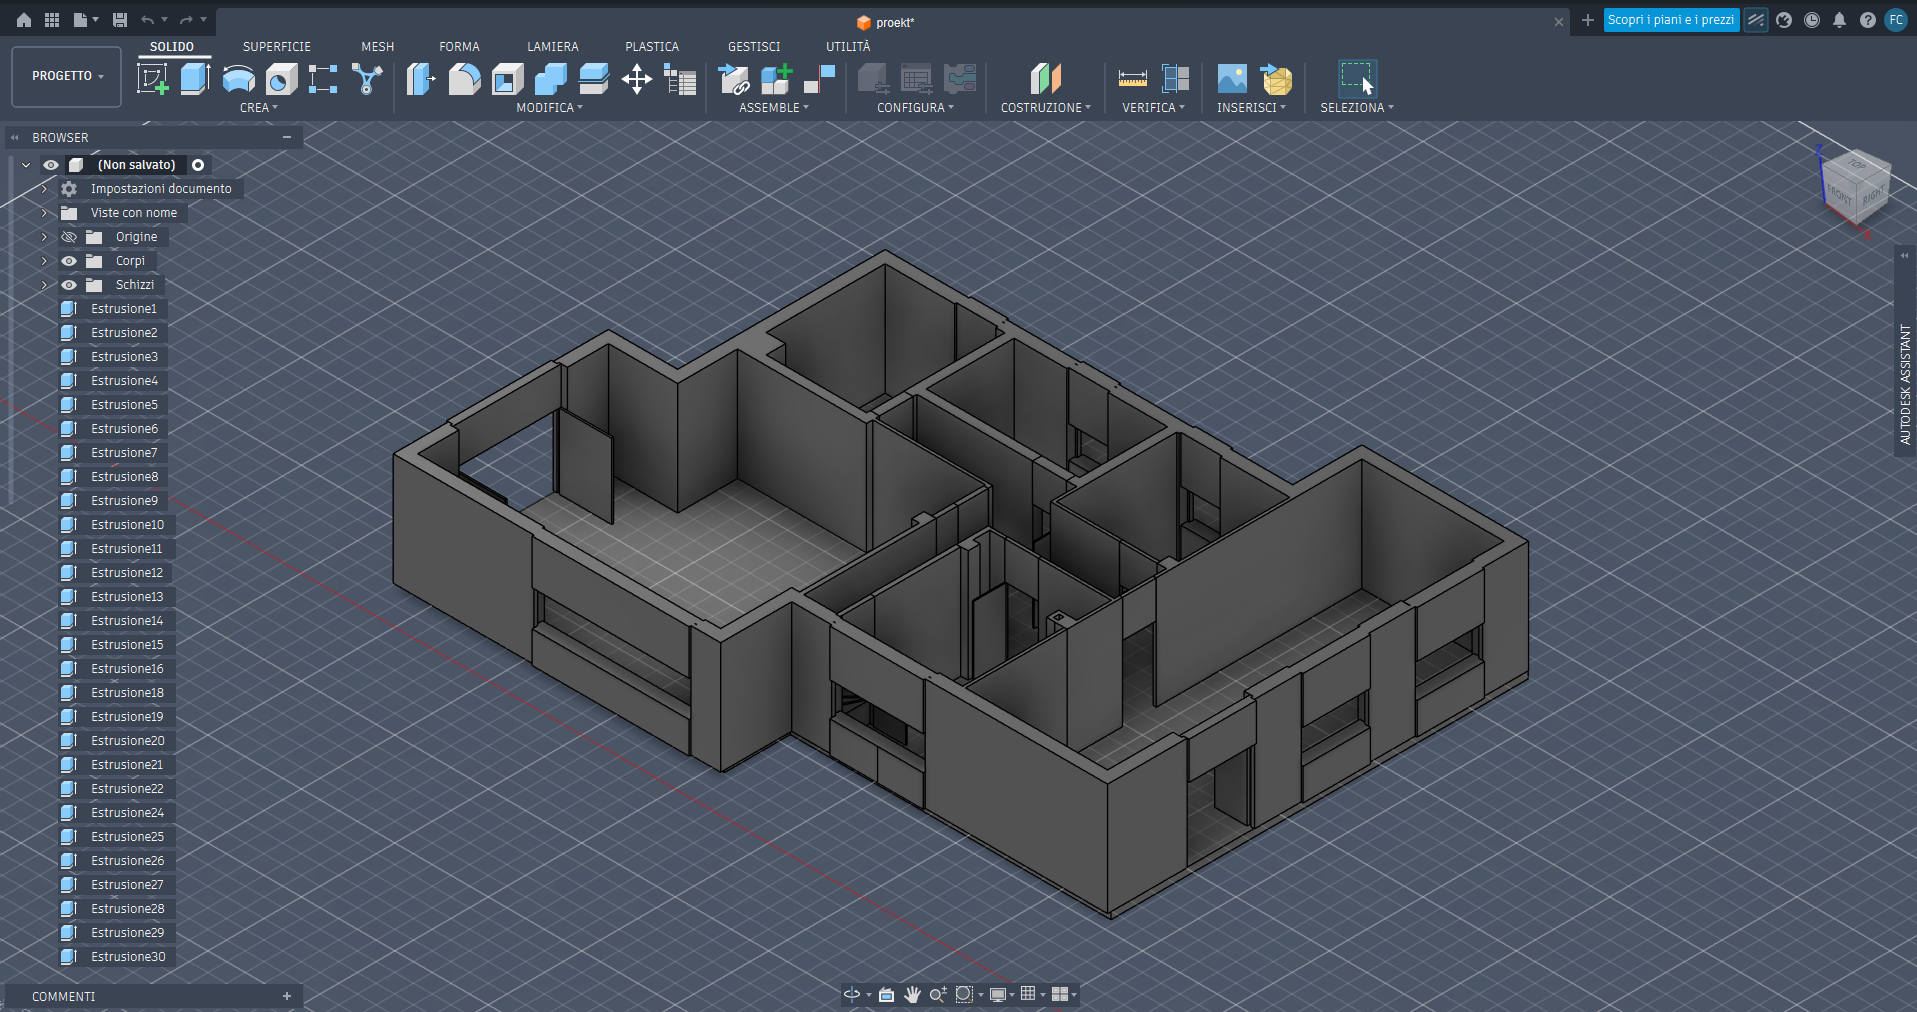
\includegraphics[width=\linewidth]{assets/screen1.png}
        \caption{Modello 3D del primo piano dell'appartamento;}\label{fig:arch1}
    \end{subfigure}
    \begin{subfigure}{0.6\linewidth}
        \centering
        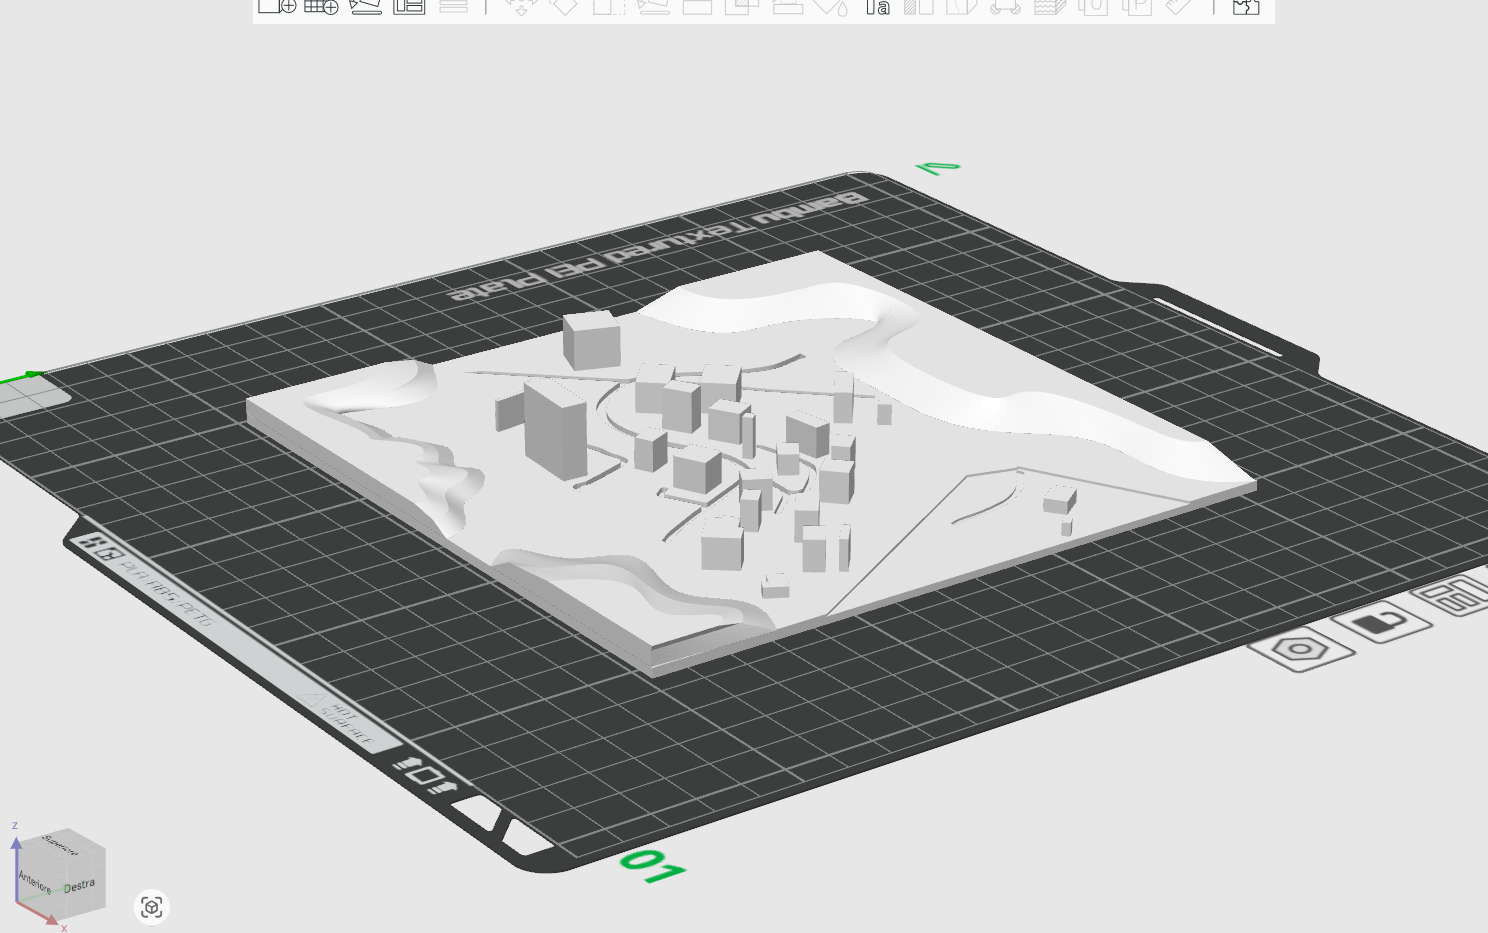
\includegraphics[width=\linewidth]{assets/screen2.png}
        \caption{Modello 3D della vista topografica dell'ubicazione dell'appartamento;}\label{fig:arch2}
    \end{subfigure}
    \begin{subfigure}{0.6\linewidth}
        \centering
        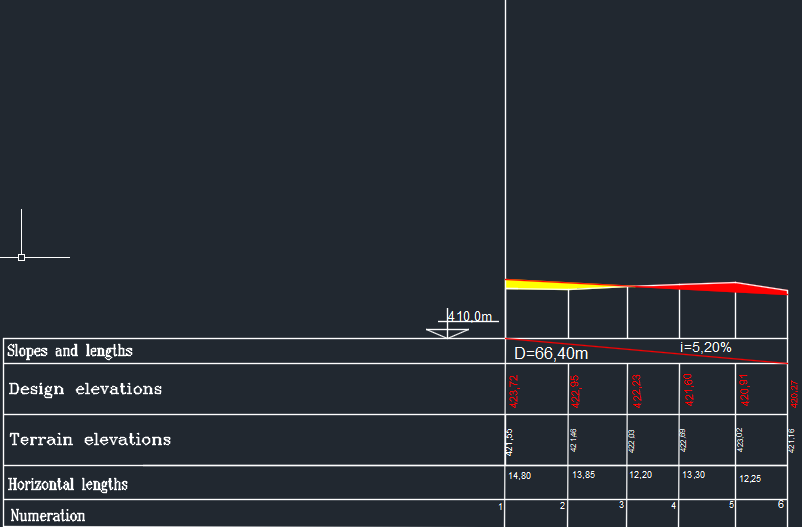
\includegraphics[width=\linewidth]{assets/screen3.png}
        \caption{Analisi delle curve di livello della zona collinare;}\label{fig:arch3}
    \end{subfigure}
    \caption{Progetto architettura e topografia.}\label{fig:arch}
\end{figure}

\progetto{Manutenzione, formazione ``Hands-on''}{Ragazzo Ungherese, Feb 2026}
L'affiancamento del tirocinante ungherese ha richiesto un approccio più individuale (one-to-one) e focalizzato sull'hardware. Piuttosto che limitarci solamente alla progettazione, lo abbiamo coinvolto attivamente nel troubleshooting e nella riparazione pratica del parco macchine del laboratorio. Insieme abbiamo diagnosticato problemi sulle stampanti 3D, effettuato il cambio di estrusori e motorini del filamento, e gestito i cablaggi. Inoltre, abbiamo utilizzato OnShape per modellare e poi stampare in 3D le componenti strutturali mancanti necessarie per completare il montaggio delle stampanti stesse, unendo così la diagnostica alla fabbricazione digitale. \\ Vedi figure \ref{fig:ung1} e \ref{fig:ung2}.
\begin{figure}
    \centering
    \begin{subfigure}{0.45\linewidth}
        \centering
        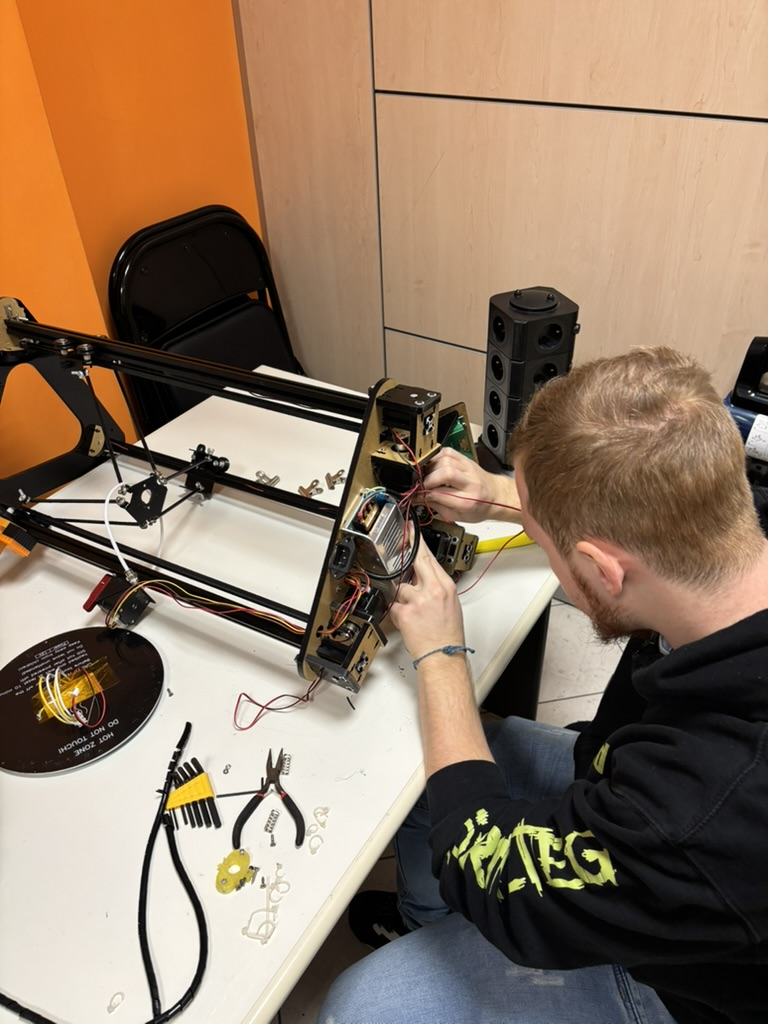
\includegraphics[width=\linewidth]{assets/A1B62198-F5B9-405B-969B-6D168E18F0CB_1_105_c.jpeg}
        \caption{}\label{fig:ung1}
    \end{subfigure}
    \begin{subfigure}{0.45\linewidth}
        \centering
        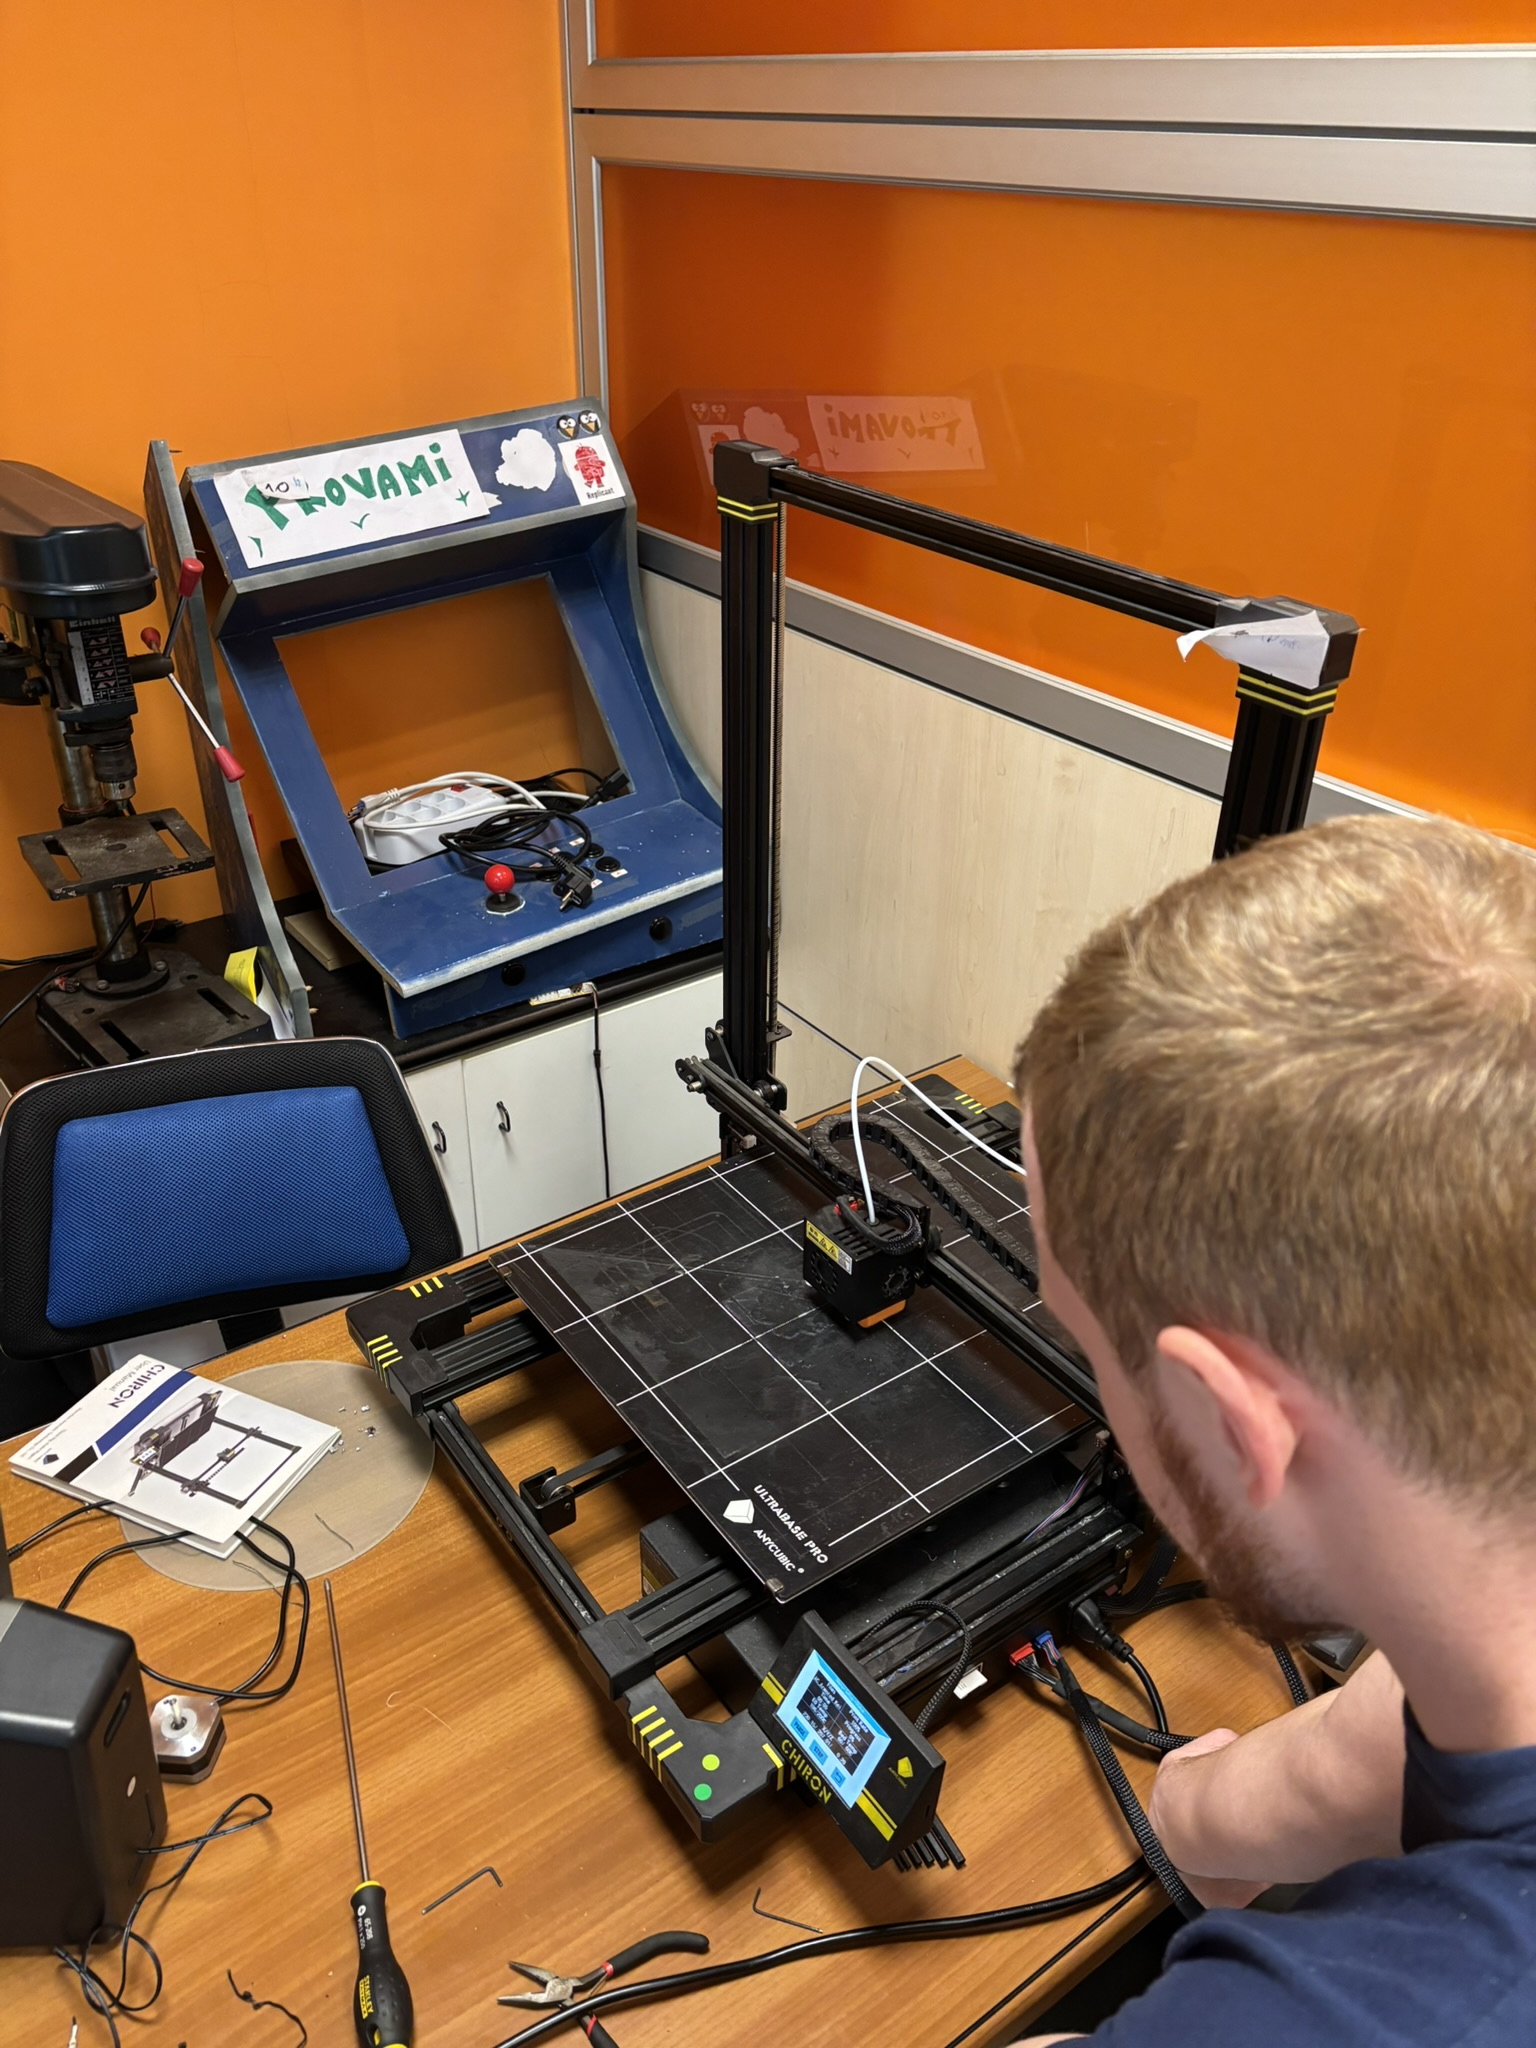
\includegraphics[width=\linewidth]{assets/088153F2-A1BA-4EF8-AC87-1DB7794AB80A_1_102_o.jpeg}
        \caption{}\label{fig:ung2}
    \end{subfigure}
    \caption{Tirocinio ragazzo Ungherese, formazione ``Hands-On''}\label{fig:ung}
\end{figure}